\chapter{Attaque SSLstrip 2}

\begin{figure}[H]
  \caption{Attaque SSLstrip 2 (diagramme Dia)}
  \fbox{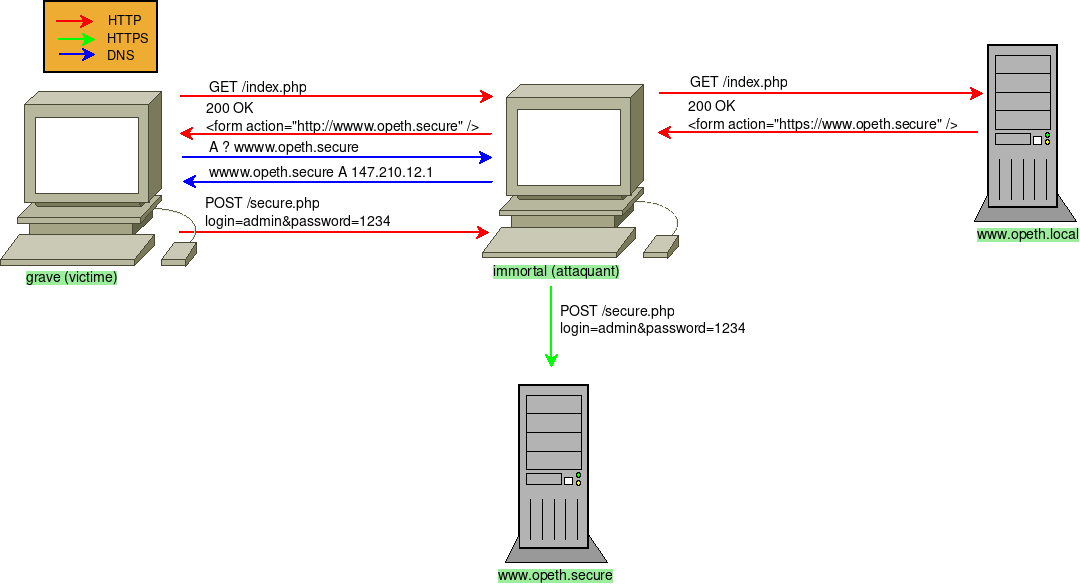
\includegraphics[width=\textwidth]{../medias/sslstrip2/attack.png}}
\end{figure}

Comme vu précédemment, une contremesure a été mise en place afin de déclarer aux clients d'un serveur qu'ils doivent utiliser une connexion sécurisée en HTTPS pour leur futures connexions avec celui-ci. Vous pouvez vous reporter à la section \hyperref[sec:hsts]{Contremesures} pour plus de précision.

Notre but est donc de contourner le HSTS en réutilisant l'attaque SSLStrip. Malheurement, on ne peut pas la réutiliser directement car le navigateur a gardé en que toutes connexions sur cette page doit se faire en HTTPS.

\section{Description de l'attaque}
Cette extension de SSLStrip a été pensée par LeonardoNve. Elle permet donc de passer au travers d'une des nouvelles contremesures mise en place sur les navigateurs. En effet, si l'attaquant se place en homme du milieu, il va pouvoir intercepter le trafic entre le client afin de faire le traiter comme suit.

Lorsque le client va se connecter au serveur sur une page HTTP, l'attaquant va modifier sur cette page en remplaçant tous les liens HTTPS en HTTP mais aussi en changeant le nom de domaine. Changer le nom de domaine changera le comportement du navigateur. En effet, comme le navigateur ne connaît pas ce nom de domaine, il n'envera pas d'exception.

Voici un exemple :

Si le lien est \verb+https://www.domain.secure+, on peut le remplacer par \verb+http://wwww.domain.secure+.

Il faut noté que l'on enlève le \verb+s+ de \verb+https+ et que l'on remplace \verb+www+ par \verb+wwww+ ce qui change bien le nom de domaine.

Ainsi, l'attaquant fait croire au navigateur que cette requête est légitime et que \verb+wwww.domain.secure+ correspond au serveur distant. La connexion sera donc en HTTP, donc en clair.

\section{Mise en place de l'attaque}

\section{L'attaque}
